\section{Modelo de despliegue}


% - - - - - - - - - - - - - - - - - - - - - - - - -
\subsection{Requerimientos no funcionales}
\begin{NFRequieriments}
\NFRitem{1}{Mantenibilidad}{
\begin{itemize}
\item Todo nuevo requerimiento funcional o no funcional debe ser platicado con el analista y arquitecto de software para poder apreciar el impacto que éste tendrá sobre el sistema y proceso de negocio.
\item Existirá un plan de mantenimiento creado por los integrantes del equipo de desarrollo que se platicará al cliente para darle a conocer los costos del mantenimiento una vez que el sistema haya sido entregado. 

\end{itemize}
}
\NFRitem{2}{Eficiencia}{
\begin{itemize}
\item Toda funcionalidad del sistema y transacción de negocio debe responder al usuario en menos de 5 segundos.
\item El sistema debe ser capaz de operar adecuadamente con usuarios conectados de una forma concurrente.
\item Los datos modificados en la base de datos deben ser actualizados para todos los usuarios que hacen consultas a ésta de una manera casi inmediata.

\end{itemize}

}
\NFRitem{3}{Seguridad}{
\begin{itemize}
\item Los datos estarán guardados en una base de datos mysql  MySQL con usuarios y contraseñas que serán cambiadas cada 6 meses. 
\item Se deben hacer respaldos semanales de la base de datos. 
\item Los formularios para ingresar datos estarán validados por tipo de dato, longitud e internamente se utilizará un ORM(Object Relational Maping) para evitar inyecciones SQL.
\item El framework que utilizaremos provee una encriptación usando Crypt. Todos los valores son encriptados utilizando OpenSSL y el cifrado AES-256-CB 

\end{itemize}
}
\NFRitem{4}{Usabilidad}{
\begin{itemize}
\item El tiempo de aprendizaje del sistema por un usuario deberá ser menor a una semana.
\item La tasa de errores cometidos por el usuario deberá ser menor del 1\% de las transacciones totales ejecutadas en el sistema.
\item El sistema debe proporcionar mensajes de error que sean informativos y orientados a usuario final.
\item El sistema debe contar con una pantalla para contacto con los desarrolladores para cualquier tipo de aclaración.
\item La aplicación web debe poseer un diseño “Responsive” a fin de garantizar la adecuada visualización en múltiples computadoras personales, tabletas y teléfonos inteligentes.
\item El sistema debe poseer interfaces gráficas bien formadas.

\end{itemize}
}
\NFRitem{5}{Dependabilidad}{
\begin{itemize}
\item El sistema debe tener una disponibilidad del 99,99\% de las veces en que un usuario intente accederlo.
\item El promedio de duración de fallas no podrá ser mayor a 15 minutos.

\end{itemize}
}
\NFRitem{6}{Extensibilidad}{
\begin{itemize}
\item El sistema podrá tener un crecimiento en el futuro ya que estará programado por módulos y esto hará más fácil su crecimiento en un futuro.
\end{itemize}
}
\NFRitem{7}{Escalabilidad}{
\begin{itemize}
\item La escalabilidad dependerá fuertemente del plan de base de datos que se esté pagando.
\end{itemize}

}
\end{NFRequieriments}
\newpage
% - - - - - - - - - - - - - - - - - - - - - - - - -
\subsection{Modelo de despliegue del sistema}

	\begin{figure}[htbp!]
		\centering
			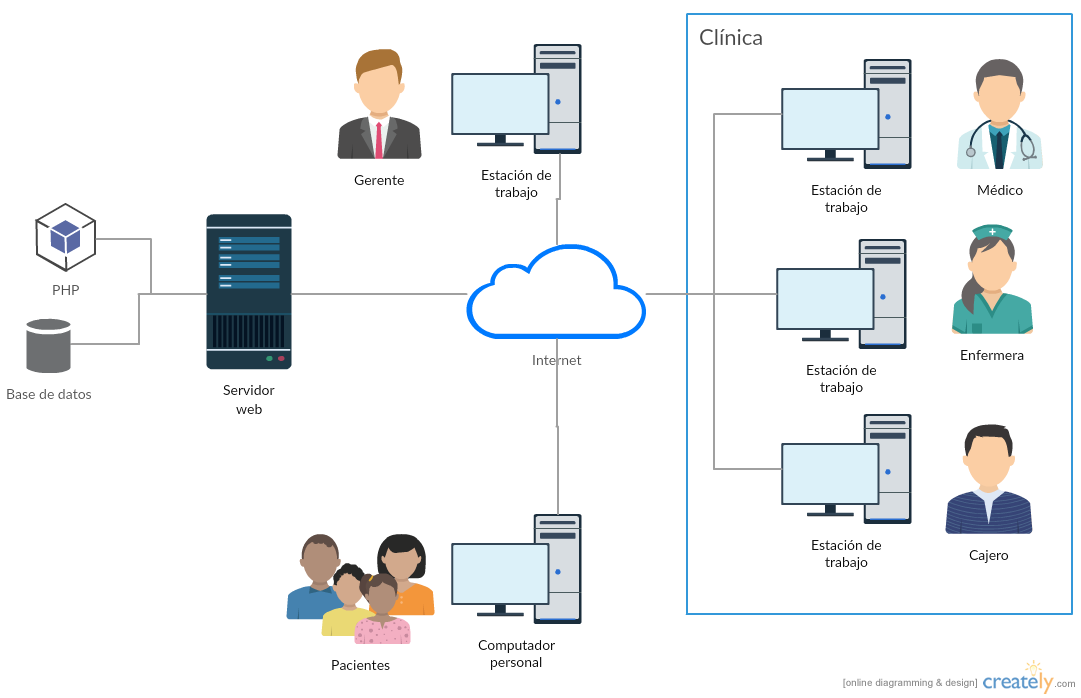
\includegraphics[width=0.8\textwidth]{images/Diagrama_despliegue}
		\caption{Diagrama de despliegue.}
	\end{figure}


% - - - - - - - - - - - - - - - - - - - - - - - - -
\subsection{Especificación de Plataforma}


\textbf{Servidor web}
\begin{enumerate}
\item \textbf{Hardware}
\begin{itemize}
\item Procesador: Intel Xeon 1220
\item RAM: 4 GB DDR3 1600 MHz
\end{itemize}
\item \textbf{Software}
\begin{itemize}
\item Sistema operativo: Debian 8 Jessie 64 bits
\item Servidor web: Apache 2
\begin{itemize}
\item Módulo PHP 5 con conector para MongoDB
\end{itemize}
\item Servidor de base de datos: MongoDB 3.2
\end{itemize}
\item \textbf{Red}
\begin{itemize}
\item Conexión a internet cableada de 20 Mb/s
\end{itemize}
\end{enumerate}

\textbf{Estación de trabajo y computadores personales}
\begin{enumerate}
\item \textbf{Hardware}
\begin{itemize}
\item Procesador: Intel Celeron N2840 o superior
\item RAM: 2 GB o superior
\end{itemize}
\item \textbf{Software}
\begin{itemize}
\item Navegador Web: Chrome 24, Firefox 24, Internet Explorer 10, Safari 7 o superior.
\begin{itemize}
\item Soporte para cookies
\end{itemize}
\end{itemize}

\item \textbf{Red}
\begin{itemize}
\item Conexión a internet de 2 Mb/s
\end{itemize}

\end{enumerate}